\chapter{\uppercase{SnipR} Fundamentals}{}
\label{sec:fundamentals}

% \fancybreak{\pfbreakdisplay}

\lettrine[lraise=0.1, nindent=0em, slope=-.5em]{T} {HIS CHAPTER} sets the stage for the complete description of the \uppercase{SnipR} in the next sections.

\section{Eager vs. Lazy Code Retargeting}
\label{sec:eagervslazy}

\uppercase{SnipR} builds on an eager code retargeting policy, a policy that is executed from the search interface. Below, this policy and its opposite---a lazy code retargeting policy, a policy that is executed at the IDE---are described.

\subsection{Eager Retargeting}

Eager retargeting is the policy of continually making code changes on one or more results, and feeding any suitability scrutiny on the outcome back into the search process\footnote{A rapid experimentation of example code}. A process that has such a policy operates under two assumptions:

\begin{enumerate}
	\item Code retargeting is a \emph{cheap}---efficient---operation, and
	\item Code retargeting ought to be done often
\end{enumerate}

Code retargeting ought to be done often in dynamic and exploratory scenarios---i.e., when the developer is working in an unfamiliar domain~\cite{Brandt:2009ew}. In such a scenario the type and number of example code may quickly change as further searches are performed. Also, if one wants to assure a rapid understanding of unfamiliar found code~\cite{Brandt:2009ew}, then it helps to frequently retarget any results to get a better picture of the result's suitability.

The expected advantages of eager retargeting are:

\begin{enumerate}
	\item The example code is more likely to match what the end user had in mind.
	\item The end user can have more confidence sooner that the picked examples were the right ones.
\end{enumerate}


\fancybreak{\pfbreakdisplay}

\subsection{Lazy Retargeting}

Lazy retargeting is the policy of only making code changes on a result at the point of integration. Under this policy, there is no guarantee---beyond relative ranking values---of the result's suitability. A process that has such a policy operates under two assumptions:

\begin{enumerate}
	\item Code retargeting is an \emph{expensive} operation, and
	\item Code retargeting ought to be done at the point of integration
\end{enumerate}

A process that has such a policy assumes code retargeting is a costly operation~\cite{Brandt:2009ew, Wightman:2012gc}. This is based on the observation that---at the point of integration---unrelated and/or unsuitable results require many more code changes than suitable results.

\fancybreak{\pfbreakdisplay}

\subsection{Reasoning about these two policies}

Intuitively, one needs to figure out whether an eager code retargeting policy leads to a \emph{cheaper} and thus \emph{faster} code search process than its opposite. 

One could model the notion of ``cost'' to retarget code examples by the following components:

\begin{enumerate}
	\item Code understanding
	\item Code modification
	\item Code disturbance
\end{enumerate}
 
The code understanding effort takes into account the time needed to carry out basic program comprehension actions, such as locating the snippet, doing content analysis, deciding which snippets to exclude. This effort is denoted by $U_{s}$, which is defined as the average effort required before starting the actual retargeting actions.

Code modification efforts represents the cost of changing the necessary tokens in a snippet. For a sequence of tokens `a', let $\alpha^{+}(a)$ and $\alpha^{-}(a)$ denote the cost of changing and rolling back `a'. This term is formulated as: 

\begin{equation}
	\alpha(S_{1}, S_{2}) = C_{s} \times (\sum_{a \in S_2 - S_1}\alpha^{+}(a) + \sum_{a \in S_1 - S_2}\alpha^{-}(a))
	\label{costmodification}
\end{equation} where $C_{s}$ is the average estimated time for one generic snippet change performed by the developer.

Code disturbance expresses the cost of tinkering when developers face a problematic situation. It is assumed that code disturbance is proportional to the amount of interruptions---e.g., unpredictable errors---experienced by a developer during retargeting and how long each interruption takes as a snippet varies. This term is formulated as:

\begin{equation}
	\epsilon(S_{j}) = T_{s} \times Interruption(S_j)
	\label{costmodification}
\end{equation} where $T_{s}$ is the average estimated time an interruption takes, $S_j$ the snippet being modified, and $Interruption(S_j)$ the number of interruptions experienced when changing a snippet $S_j$. 

Therefore, the overall retargeting cost is defined as:

\begin{equation}
	cost(S_1, ..., S_n) = U_s + (\sum_{i-1}^{n}(\alpha(S_{i-1}, S_{i}) + \epsilon(S_{i})))
	\label{totalWork}
\end{equation} where $S_1, ..., S_n$ are different snippet variations that can be derived from retargeting actions, and $S_0$ is the initial snippet.   

From the above model, one can assume that the \emph{winner} policy is the one with the smallest total cost.

Eager retargeting assumes a low cost. This is based on the observation that unsuitable results---i.e., results that cannot be retargeted---are excluded more often\footnote{i.e., the search space is reduced.}, leaving the developer only suitable choices to handle. Obviously, this will lead to a low total cost. This is because the number of interruptions and code modifications effort experienced by a developer to put a code snippet in a state that he/she is satisfied with is minimized. 

In contrast, as it has been already suggested in previous work~\cite{Brandt:2009ew, Wightman:2012gc}, a lazy retargeting policy assumes a high cost. Under this policy, it is common for one to look at each promising result (suitable or unsuitable) in its entirety\footnote{all the way to try to retarget each individual result at the IDE.}---usually one by one. If the retargeting of such result is unsuccessful, then the developer will try to explore the problem and then try all possible ways he/she can correct the problem. Not only this could lead to more frequent interruptions, more code changes and thus to a high total cost, but also to a sluggish searching interaction~\cite{Gray:2000im}.

Since the major ``cost'' of each policy is directly connected to the time spent by the developer searching for suitable code, a policy leading to a \emph{cheaper} code search process leads also to a \emph{faster} code search process.

% 
% \section{What rules should guide the Retargeting of found code?}
% \label{sec:sniprrules}
% 
% \uppercase{SnipR} models code searching as a short cycle of alternating query, screen, and retarget phases: found code is retargeted with commands issued just following to the displaying of a result set or prior to issuing a query (Figure). This model is operationalized using a state machine (Figure): during browsing, reported results are added to a queue; when the user .    
% 
% when the user edits code, all pages in the queue are assigned to new characters. 


\section{How to start developing with \uppercase{SnipR}}
\label{sec:sniprscenario}

A scenario will be given to help introduce the main interaction techniques. \uppercase{SnipR} offers two choices for interacting with code-centric sites: to issue queries and retargeting operations separately, or to intermix queries and retargeting operations. For sake of clarity, this section will focus on the former.

Olivia is an amateur developer and open source evangelist who frequently practice search-driven development at her workplace. Olivia would like to transition a sentiment analysis tool (that uses the Twitter API) to use the Facebook API. The updated tool should handle the sentiment classification of status updates in Facebook. She wants status updates to be classified dynamically. She is familiar with Java and has some Machine Learning experience, but does not consider herself an expert developer.

Olivia starts by opening Twist---a \uppercase{SnipR}-aware snippet-centric search engine she frequently visits for discovering open source libraries. This engine spans large sets of open source projects; mostly indexed from a variety of project hosting sites, such as Github, and Google code. Olivia interacts with Twist by using Twist's own language (also called Twist). This language allows Olivia to use queries and/or code retargeting operations to do code searching. The design of this language will be described in Chapter~\ref{chap:twist}. Figure~\ref{fig:twist} shows Twist's Web interface. 

\begin{figure}[!ht]
    \centering
    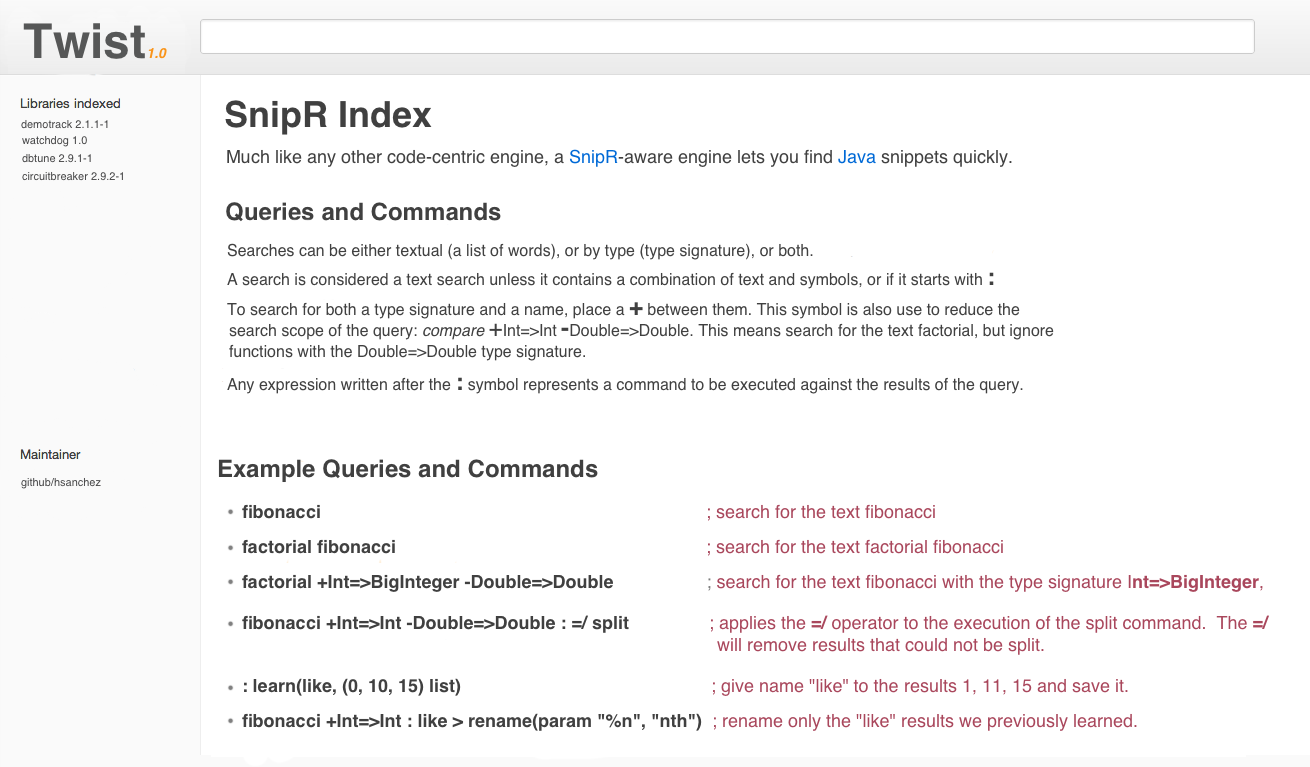
\includegraphics[width=\textwidth]{images/twistsite}
    \caption{Twist's Web Interface.}
    \label{fig:twist}
\end{figure}
% \pagebreak

To start gathering code examples, Olivia issues a query targeting Facebook APIs written in Java. Olivia specifically looks for functionality that deals with status or post updates. She does not want any android specific source code. Consequently, Olivia's first query will contain a list of words matching her intent and a reduction in search scope. Figure~\ref{fig:twistquery} shows this query and the results produced by it. 

\begin{figure}[!ht]
    \centering
    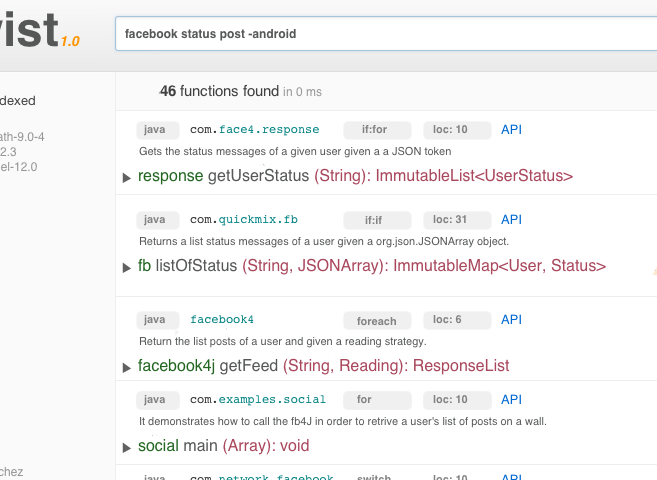
\includegraphics[width=\textwidth]{images/twistquery}
    \caption{Olvia's first query, which targets Facebook APIs written in Java.}
    \label{fig:twistquery}
\end{figure}
% \pagebreak

She tries to screen all of the results but gives up after some time. She does not have time to look at every single results. Consequently, she will use Twist's functionality to her own advantage. She issues a command that will filter out those results which size (size in terms of lines of code) exceeds 20 lines of code (Figure~\ref{fig:twistslash}). The output of this command is clearly a fewer number of results to handle. Consequently, Olivia's screening efforts will be reduced.

\begin{figure}[!ht]
    \centering
    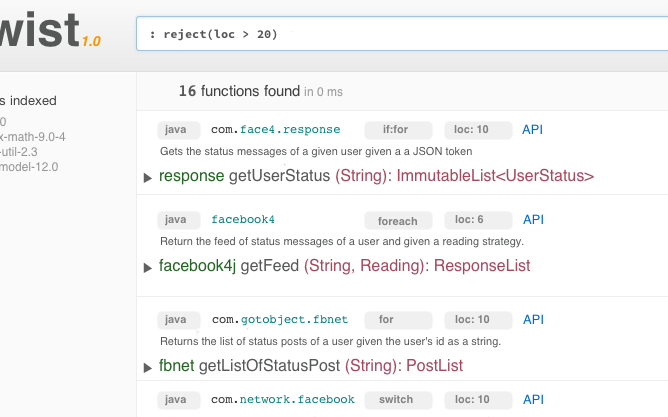
\includegraphics[width=\textwidth]{images/twistslash}
    \caption{Olivia filters out the code examples whose size exceeds 20 lines of code. The 
	 filter command takes as an input the list of current results and an anonymous function, 
	 which is applied to every result in that list.}
    \label{fig:twistslash}
\end{figure}  

Some of these results (Figure~\ref{fig:twistslash}) have highly coupled dependencies that Olivia is not interested in using, such as ImmutableList from Google Guava library. She then issues a retargeting request that will replace those dependencies with APIs found in the Java SDK. Olivia can specify these dependencies by typing an associated abbreviation; e.g., ImmutableList can be written as IL or ImL. The execution of this request reloads the Twist page, listing the successfully retargeted snippets and adding red markers next to the failed-to-retarget snippets.  These markers can point Olivia at which results she should not spend any retargeting effort from now on. Figure~\ref{fig:twistretarget} shows this command and the results produced by it\footnote{favorites is a sub list extracted from list and its defined as: learn(favorites, (0, 1, ...) list )}. 

\begin{figure}[!ht]
    \centering
    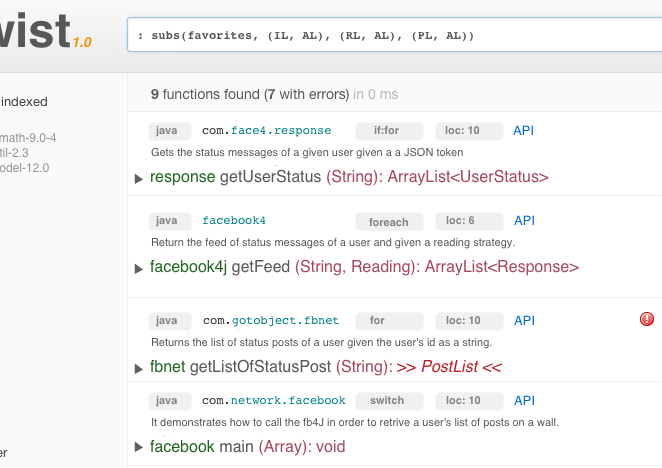
\includegraphics[width=\textwidth]{images/twistretarget}
    \caption{Olivia issues the subs command, which will replace one type for 
	 another.}
    \label{fig:twistretarget}
\end{figure} 

For Olivia, having the failed-to-retarget snippets around is distracting. Therefore, she issues another command which will drop any failed-to-retarget results from the current list of results. Figure~\ref{fig:twistclean} shows this action. 

\begin{figure}[!ht]
    \centering
    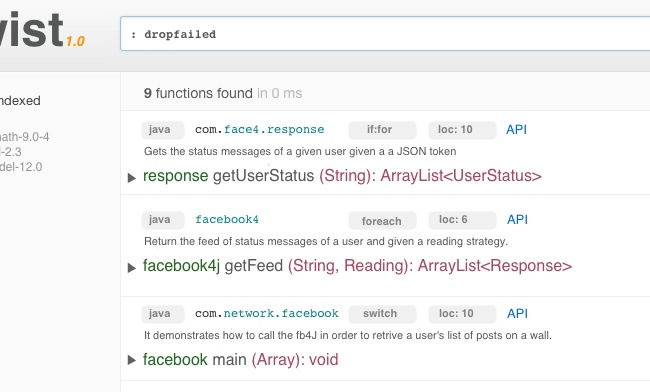
\includegraphics[width=\textwidth]{images/twistclean}
    \caption{Olivia issues a user-defined command, named dropfailed, which will drop 
	 any failed-to-retarget results from the current list.}
    \label{fig:twistclean}
\end{figure}   

She arbitrarily clicks on individual results---a result found in the result set---that she sees as promising for additional retargeting. This action offers the choice to further filtering of these results---by retargeting---to gain more confidence of these results' suitability (see Figure~\ref{fig:retargeting}). She then invokes a few additional commands: rename certain variables, and change a condition-controlled loop (e.g., for loop) to another one (e.g., while loop), matching what Olivia had in mind for how and what status updates are obtained\footnote{This process can continue (See Eager retargeting policy in Section~\ref{sec:eagervslazy}) until Olivia decides to stop.}. Again, those unsuitable results will be filtered out and thus reducing the number of results to be inspected by Olivia.

Continuing her information gathering, Olivia may continue retargeting results until there are no more results to screen or to not like any of the different variations. This can happen, which can lead Olivia to modify her previous queries to obtain similar or different results than she had previously obtained.

When she is satisfied with the resulting code example, she can evaluate these results in more detail and thus pick the most suitable example she can integrate into her own code.

